\documentclass[11pt,letterpaper]{article}
\usepackage[lmargin=1in,rmargin=1in,bmargin=1in,tmargin=1in]{geometry}
\usepackage{style}

\setlength{\parindent}{0ex}
\usepackage{mathtools} % Overlap Symbols

\usepackage{tikzsymbols}

% -------------------
% Content
% -------------------
\begin{document}

% Title
\begin{center} {\bfseries \LARGE MATH 141 --- Comment Card Responses --- Fall 2025} \end{center}

Here are select responses to comment cards given at the end of class. When computed, the class rating (out of 10) is given. The comment (often paraphrased for clarity) is given in italics/bold with the response following the comment. The responses are labeled by class date---with the class topic given. The classes are given in reverse-chronological order for ease of access to the most recent class. You may also click any of the hyperlinks below to jump to that date.

\begin{itemize}
\item \hyperref[09-10]{09/10, Wednesday: Product \& Quotient Rule}
\item \hyperref[09-08]{09/08, Monday: Derivative Rules \& Chain Rule}
\item \hyperref[09-05]{09/05, Friday: Derivative Definition}
\item \hyperref[09-03]{09/03, Wednesday: Continuity}
\item \hyperref[08-29]{08/29, Friday: Limit Techniques}
\item \hyperref[08-27]{08/27, Wednesday: Limit Techniques}
\item \hyperref[08-25]{08/25, Monday: Limit Techniques}
\item \hyperref[08-22]{08/22, Friday: Limit Techniques}
\item \hyperref[08-20]{08/20, Wednesday: Graphical Limits}
\end{itemize}

% 09/10, Wednesday: Product \& Quotient Rule
\newpage
\section*{09/10, Wednesday: Product \& Quotient Rule\label{09-10}}

\begin{itemize}
\item {\bfseries\itshape Class Rating:} 9.25/10
\item {\bfseries\itshape What are some of the applications of derivatives?} Don't worry, we will get to them! Although, we will only begin to scratch the surface this semester. I am always more than happy to discuss more of them outside of class. 

\item {\bfseries\itshape I don't like product rule having embedded chain rules} Just you wait, we'll have even more rules happening all at once! But don't worry, we build there slowly so you will have the skills by the time we get to those. Luckily, the derivative we do `in a vacuum' are often harder than the ones we work with in practice.

\item {\bfseries\itshape It's hard for me to tell when to use the chain rule} You can always use the chain rule! For example, if I wanted the derivative of $\sin x$, you might think, ``That's just $\cos x$.'' Correct! But I can even think of that as coming from the chain rule: the derivative of $\sin$ is $\cos$, so we have $\cos x$ but then I have to multiply by the derivative of the `next layer down', which is $x$. The derivative of $x$ is 1. So, the derivative should be $\sin x \cdot 1= \sin x$. There is never any harm in applying it so long as you do correct things! Over time, you will become more confident in when you need it and when you don't. 







\item {\bfseries\itshape Thanks for making this simple!}
\item {\bfseries\itshape Do you have to solve anything for quotient rule?}
\item {\bfseries\itshape Since I'm squared, I'll be fair}
\item {\bfseries\itshape Giga chad}
\item {\bfseries\itshape Alt+$\mathrlap{\text{\textbackslash}}{\mathcal{U}}$Fu=\$}
\item {\bfseries\itshape Genuinely thank you for the simple versions of product/chain/quotient rules!}

\item {\bfseries\itshape \dots Math just sucks}
\item {\bfseries\itshape Thanks!}
\item {\bfseries\itshape Hidy lowdy, lowdy what?}
\item {\bfseries\itshape I was genuinely really confused. I will attend your office hours}
\item {\bfseries\itshape Is there an SI for this class?}
\item {\bfseries\itshape Your weird ass quotient rule thing was helpful}
 \item {\bfseries\itshape You gave two different formulas to solve the same problem}
 \item {\bfseries\itshape I wish I knew we would cover this before I did the HW\dots}

\item {\bfseries\itshape you pookie}
\item {\bfseries\itshape lo di high, high di lo}
\item {\bfseries\itshape Thanks for the quotient rule}
\item {\bfseries\itshape Rules + stuff}
\item {\bfseries\itshape Hey}
\item {\bfseries\itshape Very silly}
\item {\bfseries\itshape Why do you wear glasses, you seem like a bifocal guy}
\end{itemize}

% 09/08, Monday: Derivative Rules \& Chain Rule
\newpage
\section*{09/08, Monday: Derivative Rules \& Chain Rule\label{09-08}}

\begin{itemize}
\item {\bfseries\itshape Class Rating:} 9.14/10
\item {\bfseries\itshape Is email the best method of contact?}
\item {\bfseries\itshape Could you help us understand the definition and functions of derivatives more?}
\item {\bfseries\itshape What are other examples of continuous functions that are not differentiable?} 
\item {\bfseries\itshape Will the exam study guide be posted to Blackboard?}
\item {\bfseries\itshape I am struggling with limits on the homework, especially evaluating what the limit is from left or right side. Which video/lectures do you recommend going over?}
\item {\bfseries\itshape Life saver with the box method. Thank you!}
\item {\bfseries\itshape I don't like the chain rule}
\item {\bfseries\itshape It was a little fast paced}
\item {\bfseries\itshape I liked your chain rule method}
\item {\bfseries\itshape I liked the box method.}
\item {\bfseries\itshape Box method was great!}
\item {\bfseries\itshape Thank you for being a good calc teacher :P }
\item {\bfseries\itshape The Shrek Rule was helpful}
\item {\bfseries\itshape F**k da chain rule}
\item {\bfseries\itshape Thank you for being the best teacher I've had}
\item {\bfseries\itshape 1. Wall-E 2. The Incredibles 3. Inside Out} 
\item {\bfseries\itshape How do you get your coffee?} 
\item {\bfseries\itshape What is your favorite cheesecake?}
\item {\bfseries\itshape Do you like Steven Universe?}
\item {\bfseries\itshape Futurama ending has nothing over Attack on Titan}
\item {\bfseries\itshape $\uparrow\uparrow\downarrow\downarrow\leftarrow\rightarrow\leftarrow\rightarrow$ABstart}
\item {\bfseries\itshape You like rolling a lot. I agree.}

\end{itemize}

% 09/05, Friday: Continuity
\newpage
\section*{09/05, Friday: Derivative Definition\label{09-05}}

\begin{itemize}
\item {\bfseries\itshape Class Rating:} 9.07
\item {\bfseries\itshape Can we use the power rule?}
\item {\bfseries\itshape Is $\tfrac{f(x + h) - f(x)}{h}$ always used? Do we memorize this?}
\item {\bfseries\itshape Can you explain the other approaches of the derivatives?} 

\item {\bfseries\itshape I liked this better than the already printed packets}
\item {\bfseries\itshape I am retaking this course \& you explain this better than my previous teachers so thank you :) }
\item {\bfseries\itshape My last calculus professor made me drop out because of how horribly he `taught' us derivatives} 
\item {\bfseries\itshape You spoke slower!}
\item {\bfseries\itshape It was helpful to see the derivative background. I'd forgotten}
\item {\bfseries\itshape I have never had derivatives explained like this before. It was super helpful!}
\item {\bfseries\itshape More practice on derivatives please}
\item {\bfseries\itshape Why can't we just skip to the shortcut part?}
\item {\bfseries\itshape You were helpful babe}
\item {\bfseries\itshape Nothing was unhelpful sweet cheeks}
\item {\bfseries\itshape You are the goat}
\item {\bfseries\itshape Any fun plans this weekend?}
\item {\bfseries\itshape You're like batman but instead of fighting crime you teach math and ramble} 
\item {\bfseries\itshape Watch the movie Creep on Netflix}
\item {\bfseries\itshape The beginning was kind of confusing, but the end started to make sense.}
\item {\bfseries\itshape Your energy and charisma are most helpful} 
\item {\bfseries\itshape Have a great weekend goat}
\item {\bfseries\itshape I want cheesecake} 
\item {\bfseries\itshape Do you actually read these? Draw a smiley on Monday on the board if you do.}
\item {\bfseries\itshape I'm watching Jujutsu Kaisen---it's awesome} 
\item {\bfseries\itshape Do a Morgan Freeman impression}  %“Now, I know what you were expecting. A certain sound. A certain rhythm. That voice, warm as honey and steady as the earth itself. But let me tell you something… I’m not here to be Morgan Freeman. I’m here to tell you, in my own way, that no voice—no matter how beloved—can be borrowed and worn like a costume.
%
%You see, what makes him unique is not just his cadence, or his timbre, or even the way he can turn the simplest line into scripture. It’s that he is himself. And I? Well, I am me.
%
%So no… I won’t give you a Morgan Freeman impression. Instead, I’ll give you the truth: we don’t need to imitate greatness when we can speak in our own voices. And who knows? Maybe, just maybe, that’s how new legends are born.”

%“I know what you’re waitin’ for. That voice. The one folks say could make a grocery list sound like poetry. But that ain’t what you’ll find here. I won’t pretend to be him. All I can do is speak plain, in my own way… and maybe that’s enough.”

% Dont wait. Hope is a dangerous thing.
% I have no idea what those two italian ladies were singing about. Truth is, I don't want to know. Some things are best left unsaid.
% I find I'm so excited, I can barely sit still or hold a thought in my head. I think it's the excitement only a free man can feel, a free man at the start of a long journey whose conclusion is uncertain. I hope I can make it across the border. I hope to see my friend and shake his hand. I hope the Pacific is as blue as it has been in my dreams. I hope.
\item {\bfseries\itshape How tf are spheres 2-dimensional? Please elaborate} 
\item {\bfseries\itshape If there are infinitely many numbers between 0 and 1 and between 1 and 2, why isn't the amount of numbers between 0 and 2 bigger but isn't it also infinite?}

\end{itemize}

% 09/03, Wednesday: Continuity
\newpage
\section*{09/03, Wednesday: Continuity\label{09-03}}

\begin{itemize}
\item {\bfseries\itshape Class Rating:} 8.78/10
\item {\bfseries\itshape The Gateway video helped a great amount, thank you.}
\item {\bfseries\itshape Do we need to show work for every step?} 
\item {\bfseries\itshape When is the exam?}
\item {\bfseries\itshape Are the tests in-person and do we have longer than 50~minutes?} 
\item {\bfseries\itshape Will we cover squeeze theorem? We went over it in recitation} 
\item {\bfseries\itshape Does attendance in recitation affect grades?}
\item {\bfseries\itshape What is the format of the exam?} 
\item {\bfseries\itshape I need help preparing for the exam}
\item {\bfseries\itshape Maybe explain problems like `Find $a, b$ so that $f(x)$ is continuous'} 
\item {\bfseries\itshape Please draw more quick graphs that helps visualize a lot}
\item {\bfseries\itshape I liked the interaction in class}
\item {\bfseries\itshape Is the exam multiple choice or only given questions? Or a mixture?} 
\item {\bfseries\itshape Can we do more of these problems in class? More continuity?} 
\item {\bfseries\itshape Not excited for note taking} 
\item {\bfseries\itshape One of the easier lectures to understand}
\item {\bfseries\itshape I liked this}
\item {\bfseries\itshape Thanks for telling us what we need to know}
\item {\bfseries\itshape I found the examples extremely helpful.} 
\item {\bfseries\itshape Just the overall way you teach is super helpful} 
\item {\bfseries\itshape I hated the anime discussion. I hate anime and will never watch it.} 
\item {\bfseries\itshape Is Attack on Titan peak anime?}
\item {\bfseries\itshape ``Ah, dungeon food'' winged lion, Dungeon Meshi} 
\item {\bfseries\itshape You know Ball (Frieren)} 
\item {\bfseries\itshape AOT is the best show and anime ever made, if you disagree you're a child} 
\item {\bfseries\itshape Inuyasha > Frieren} 
\item {\bfseries\itshape Favorite Frieren character?} 
\end{itemize}

% 08/29, Friday: Limit Techniques
\newpage
\section*{08/29, Friday: Limit Techniques\label{08-29}}

\begin{itemize}
\item {\bfseries\itshape Class Rating:} 9.11/10
\item {\bfseries\itshape Where are the extra videos on Blackboard you said you would post that are really slow videos explaining everything?} 
\item {\bfseries\itshape Thank you for not making people feel dumb when they ask questions}
\item {\bfseries\itshape Why did we do a lab for the first lab class and then yesterday's class was all limit review?}

\item {\bfseries\itshape Where can we find extra practice problems for learned concepts?}
\item {\bfseries\itshape When is the first quiz?}
\item {\bfseries\itshape Have you ever used Bobo Botn Eastsdc"}
\item {\bfseries\itshape This was explained well!}
\item {\bfseries\itshape I suck at this}
\item {\bfseries\itshape Today was an ah-ha day}
\item {\bfseries\itshape How can I apply Calculus to Physics or simulation context?} 
\item {\bfseries\itshape Thanks for a great first full week of classes. This has actually been my favorite class so far. Have a great weekend.} 
\item {\bfseries\itshape Do we get a study guide for the exam?}
\item {\bfseries\itshape Are there any dropped check-ins?}
\item {\bfseries\itshape Will we have a review day before the exam?}
\item {\bfseries\itshape Do your research on LeBron Bymon James, aka King James}
\item {\bfseries\itshape Na, great lecture!}
\item {\bfseries\itshape Everything today clicked for me so very good} 
\item {\bfseries\itshape This was very cool! Examples were the best!}
\item {\bfseries\itshape Can we get a full lesson recap before our exams, in-person or online?}
\item {\bfseries\itshape Chipotle is not that good}
\item {\bfseries\itshape The best selling sandwich in England is the the BLT which includes both a fruit and a vegetable}
\item {\bfseries\itshape You lack ball knowledge}
\item {\bfseries\itshape Jalen hurts or Justen bulbert} 
\item {\bfseries\itshape I get within 10~km on Geoguesser}
\item {\bfseries\itshape How many languages do you speak?}
\item {\bfseries\itshape Chipotle servings have gotten too small}
\item {\bfseries\itshape Chipotle is the best}
\item {\bfseries\itshape Dap me up} % Image
\item {\bfseries\itshape Skyline is the best fast food! I'm from Cincinnati} 

\end{itemize}

% 08/27, Wednesday: Limit Techniques
\newpage
\section*{08/27, Wednesday: Limit Techniques\label{08-27}}

\begin{itemize}
\item {\bfseries\itshape Class Rating:} 8.81
\item {\bfseries\itshape There are a lot of different ways to solve limits.}
\item {\bfseries\itshape I don't know when to use each type of limit}
\item {\bfseries\itshape I am guessing 6.5/10 doesn't count for the Gateway?}
\item {\bfseries\itshape When is the second Gateway?}
\item {\bfseries\itshape You Rick rolled me on Blackboard}
\item {\bfseries\itshape Math is hard}
\item {\bfseries\itshape It was all understandable today!}
\item {\bfseries\itshape I would appreciate more algebra explanation on cancelling numbers to `make it work' for $e$ limits}
\item {\bfseries\itshape Mask made it harder to hear}
\item {\bfseries\itshape Feel better soon!}
\item {\bfseries\itshape You da man}
\item {\bfseries\itshape What do you enjoy about [?]} 
\item {\bfseries\itshape Get well soon!}
\item {\bfseries\itshape Thank you for the Gateway video!}
\item {\bfseries\itshape Confused most of the time but it comes together in the end}
\item {\bfseries\itshape This wasn't as confusing and as complicated as the last class}
\item {\bfseries\itshape Do you watch anime or only live TV?}
\item {\bfseries\itshape I like your `dumb' analogies}
\item {\bfseries\itshape Python sucks}
\item {\bfseries\itshape Yooooooo}
\item {\bfseries\itshape You should try hockey, it's like polo with more fights and more missing teeth}
\item {\bfseries\itshape Get well soon!}
\item {\bfseries\itshape You remind me of a hyperactive Yorkie} % certain set of skills
\end{itemize}

% 08/25, Monday: Limit Techniques
\newpage
\section*{08/25, Monday: Limit Techniques\label{08-25}}

\begin{itemize}
\item {\bfseries\itshape Class Rating:} 8.63/10
\item {\bfseries\itshape Do we need a calculator for this class?} Nope! In fact, none is even allowed. 
	\begin{figure}[H]
	\centering
	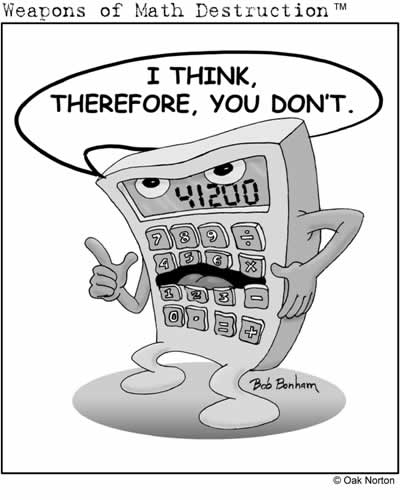
\includegraphics[width=0.2\textwidth]{images/calculator.jpg}
	\end{figure}

\item {\bfseries\itshape How do I know which homework correlates with each class period/lesson?} By the title, which should approximately correspond to the lecture titles. But you can always ask and I am happy to point it out!

\item {\bfseries\itshape Could you go over all the steps? Sometimes you skip steps} I try to balance this. I don't want to show so many that we take a lot of time and then don't cover things or see less problems. But I do not want to skip so much that I lose everyone. I try to show enough that I keep the vast majority of the room---though it may lose some folks. You can always go back in later and try to fill in the missing steps. Indeed, this is how you get better at the algebra!

\item {\bfseries\itshape Where can I practice limit problems?} Homeworks! Always start there. Beyond that, there are tons of extra problems broken down by topic in the `External Resources' folder on Blackboard. 

\item {\bfseries\itshape How do you remember and especially identify when we see certain problems?} That is the hard part---knowing which type of limit is which. There are some rules of thumb. However, this mostly comes down to experience. So, you need to do enough problems until you get a `feel' for it! 

\item {\bfseries\itshape If there were a campus shooting, where would we hide?} The general guidelines are run, hide, fight. Meaning, generally your first goal is to leave the area, not necessarily hide. This would then depend on the area---either towards center campus or across the bridge. In the classroom, that would be against the windows or chalkboard for hiding. And fight is always the last resort. You may always contact public safety if you want to know more of their guidelines for campus safety. 

\item {\bfseries\itshape You're my knight in shining armor} 
	\begin{figure}[H]
	\centering
	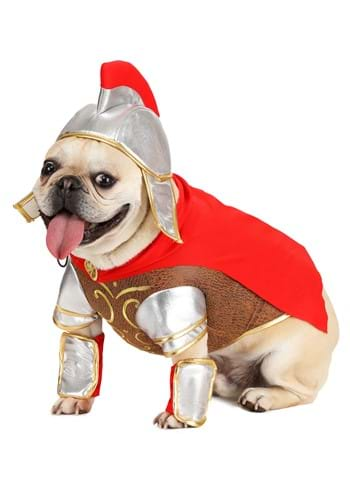
\includegraphics[width=0.15\textwidth]{images/pugcostume}
	\end{figure}

\item {\bfseries\itshape Are all the notes for the semester posted to Blackboard?} Indeed, they are! Also, the lecture videos are all posted---all broken down by lecture and labeled by the section.

\item {\bfseries\itshape Will points be taken off if we don't show the exact steps you show?} That depends on the steps. Generally, skipping some small algebra steps are fine. Skipping lots is bad. Skipping Calc steps is very bad. 

\item {\bfseries\itshape Should we know the unit circle?} Indeed! You should know all the trig functions value on the entire unit circle. There are resource videos on this in Blackboard to help!

\item {\bfseries\itshape How did you go from $\tfrac{\frac{1}{h + 5} - \frac{1}{5}}{h}$ to $\tfrac{\tfrac{5 - (h + 5)}{5(h + 5)}}{h}$?}
	\[
	\dfrac{\frac{1}{h + 5} - \frac{1}{5}}{h}= \dfrac{\frac{1}{h + 5} \cdot \frac{5}{5} - \frac{1}{5} \cdot \frac{h + 5}{h + 5}}{h}= \dfrac{\frac{5}{5(h + 5)} - \frac{h+5}{5(h + 5)}}{h}= \dfrac{\;\;\frac{5 - (h + 5)}{5(h + 5)}\;\;}{h}
	\]

\item {\bfseries\itshape Well explained!} Thanks! I tried!

\item {\bfseries\itshape Confused about the last limit with $e$} We will see more examples next class!

\item {\bfseries\itshape The examples are so helpful} There are plenty more in the homework \Winkey

\item {\bfseries\itshape Liked the werk method} Glad that you liked it!
	\begin{figure}[H]
	\centering
	
\includegraphics[width=0.25\textwidth]{images/werk.jpeg}
	\end{figure}

\item {\bfseries\itshape I would prefer to write my own notes} Never fear! We will only work from the packets for so long. After that, you will be expected to take your own notes.

\item {\bfseries\itshape Very helpful!} Thanks!

\item {\bfseries\itshape I'm looking forward to the semester} Thanks! Looking forward to working with you all!

\item {\bfseries\itshape I liked the lecture a lot I learned this concept in AP Calc and it was good way of teaching it. Also good emphasis on mental health} Thanks! Remember, the mental health sheet is on Blackboard so that you can always print more of them or click the links. Also, the resources are linked. 

\item {\bfseries\itshape People have been talking about homework being due but I don't see any due until September} I mentioned this in the syllabus video. All the homework is due two days before the exam. [So, students putting it off don't pull an all nighter right before an exam.] This schedule allows you to self pace or take breaks to focus on other courses or just a break. However, this means you have to keep track of pacing! I would suggest doing homeworks as soon as we finish the topics. 

\item {\bfseries\itshape Just gotta practice} Indeed! That is how you succeed in Mathematics. 

\item {\bfseries\itshape Please write a control of the problem and another that you work off of} I can try to remember. However, I do problems in-class essentially as I would like to see them done on exams. 

\item {\bfseries\itshape You contradicted some past statements} I did not. Which does that seem like?

\item {\bfseries\itshape You over-explained} I'm sorry. But I'd also rather go over than under!

\item {\bfseries\itshape Way better than my HS teacher!} Thanks!

\item {\bfseries\itshape Special limits was so friggin' tuff} It's fine to find things hard! Math can take some time to sit with stuff and practice. It's about the perseverance, not getting it right away. Of course, if things still don't sink in, please, ask questions, stop by for help, seek out the resources available to you! I want you to succeed!

\item {\bfseries\itshape I liked how you do an example and then we do a practice problem} I try to build in as much problem time as we can. But for some topics, that can be tough. 

\item {\bfseries\itshape You good baby girl}
	\begin{figure}[H]
	\centering
	
\includegraphics[width=0.20\textwidth]{images/blush.png}
	\end{figure}

\item {\bfseries\itshape You Rick rolled me :| } I was actually reading an article on Math Education and they had mentioned things like this as a method of student interaction. Overall, the article was really interesting and gave some nice insights into teaching and the student learning process. It's well worth checking out, \href{https://www.youtube.com/watch?v=dQw4w9WgXcQ}{http://mathworld.wolfram/math\_education/building-student-trust-and-engagement-in-the-classroom}

\item {\bfseries\itshape Still need help with conjugation!} You should hopefully do practice in recitation. There's also similar homework problems and also remember all the help resources available! 

\item {\bfseries\itshape What are different ways to memorize these?} Memorize what? The special limits? Not really that I can think of. But there's only 3!

\item {\bfseries\itshape Caleb, you talk very fast} I am sorry! It's who I am. Be comforted that most students do adjust to the cadence over time, just as one would with an accent. 

\item {\bfseries\itshape Favorite professional sports team?} I don't do sports. 

\item {\bfseries\itshape 67!} Easy, 36471110918188685288249859096605464427167635314049524593701628500- 267962436943872000000000000000.

\item {\bfseries\itshape Mandiballs} Mandibles?

\item {\bfseries\itshape $0 \cdot \infty= 1$???} Infinity is not a number, it has to come from a limiting process. So, depending on how the 0 and $\infty$ come about, yes, this is possible. We shall see this later in the course. Although, I believe I gave brief examples in lecture. 

\item {\bfseries\itshape You gotta watch a trailer for Weapons} Oh, there hasn't been a decent horror movie in years. Last one that was worth anything that I recall was The Witch. Although, Megan gave me a decent laugh. 

\item {\bfseries\itshape Recommended movies?} Oh, that really depends on what you're like and looking for. 

\item {\bfseries\itshape It's crazy how you kept track of every movie and TV show that you've ever watched, presumably since childhood} It's not as hard as you think. As of now, 2,986 movies and TV shows.

\item {\bfseries\itshape Least favorite food?} Liver.

\item {\bfseries\itshape You scare me} Now I know I'm not the best looking person, but to say that my looks are scary----how rude! But honestly, I don't judge and I'm here to help for as long as I have the time and you have the motivation to keep going!

\item {\bfseries\itshape I still think you look like Ian Hecox} We've covered this!
	\begin{figure}[H]
	\centering
	
\includegraphics[width=0.15\textwidth]{images/handsomesquidward.jpg}
	\end{figure}

\item {\bfseries\itshape Thank god for Project Runway} I've never actually seen it\dots

\item {\bfseries\itshape Are you into DND?} I've never played. Does not seem to be my thing. But I really like Baldur's Gate.
	\begin{figure}[H]
	\centering
	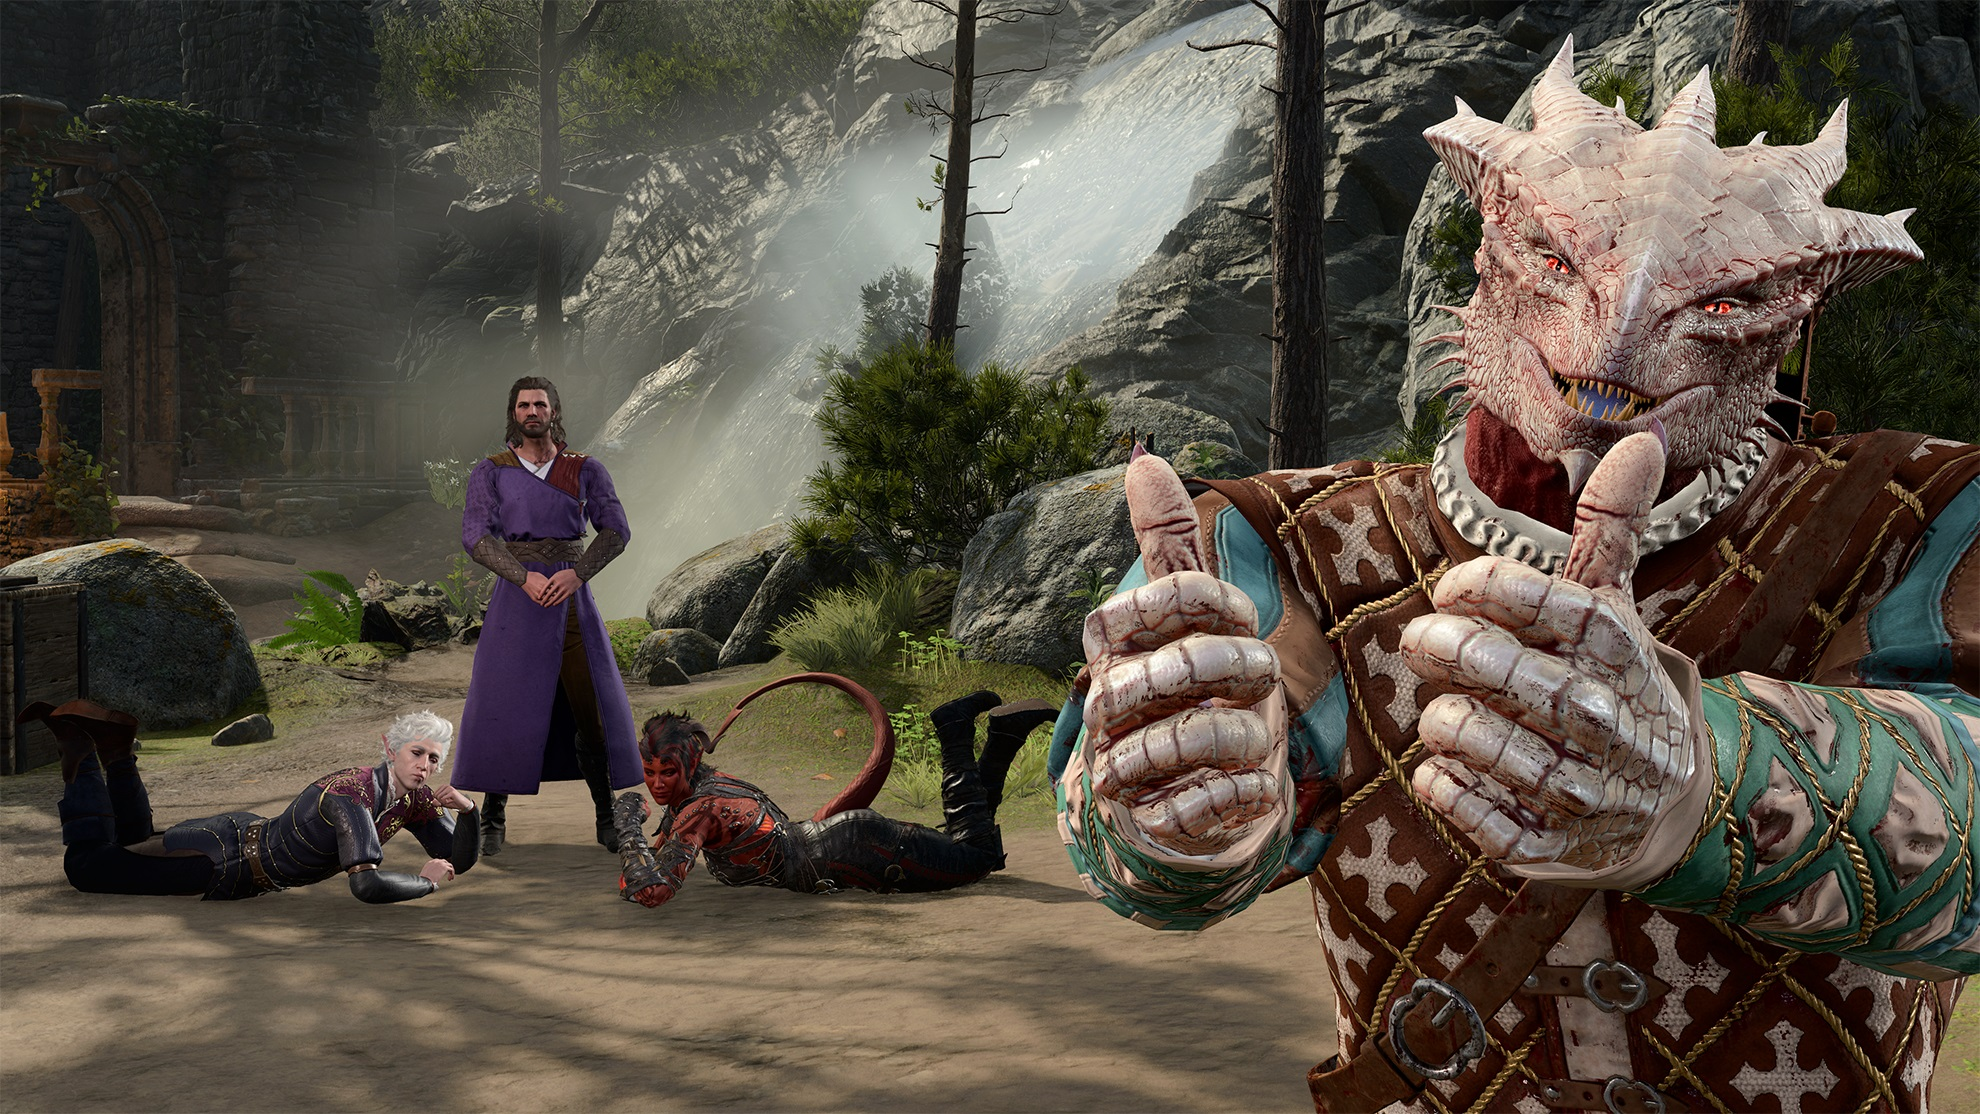
\includegraphics[width=0.365\textwidth]{images/baldur.jpg}
	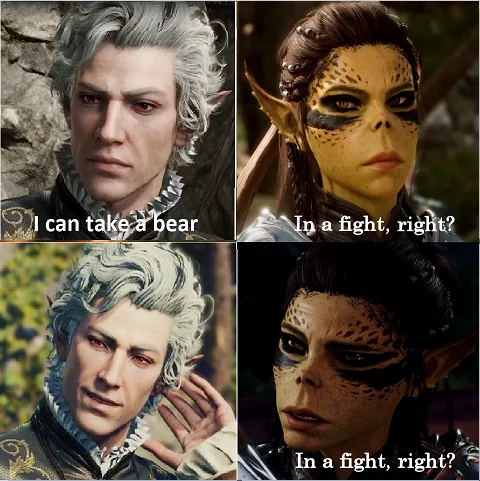
\includegraphics[width=0.25\textwidth]{images/baldur2.png}
	
\includegraphics[width=0.36\textwidth]{images/baldur3.png}
	\end{figure}

\item {\bfseries\itshape Why was 6 afraid of 7?} You're probably thinking because 7 ate (8) 9. But 6 has a greater fear after Fibonacci informed 6 that 5 ate (8) 13. 
	\begin{figure}[H]
	\centering
	
\includegraphics[width=0.15\textwidth]{images/handsomesquidward.jpg}
	\end{figure}

\item {\bfseries\itshape What's your favorite word in German?} Genau or perhaps uberlassen.
\end{itemize}

% 08/22, Friday: Limit Techniques
\newpage
\section*{08/22, Friday: Limit Techniques\label{08-22}}

\begin{itemize}
\item {\bfseries\itshape Class Rating:} 8.92/10

\item {\bfseries\itshape What's the point of the Python labs?} The department feels seeing some programming and `experiencing' the Calculus is important. Although, this (insofar as I am aware) comes from the School of Engineering. 

\item {\bfseries\itshape How do you plug in $\infty$ into a limit?} You don't! But you often do need to think about what happens when $x$ becomes infinitely large to compute some limits. Remember, $\infty$ is not a number. 

\item {\bfseries\itshape Will I need to know things like $\arctan$ for exams because I passed the gateway without it but I have never been taught it.} Though it likely won't show up often, you are expected to know the inverse trig function values. 

\item {\bfseries\itshape What is the best tool to use to brush up on my trig. values, inverse, etc. precalc stuff?} For trig, I think that I have everything you'd need on Blackboard. As for the algebra stuff, I'm not quite sure. Even Khan Academy or OrganicChemTutor might be sufficient for the course. 

\item {\bfseries\itshape What is the difference between DNE and undefined?} A limit does not exist if the right or left hand limit does not exist or they do not `align'. A function is undefined a value if it does not have a value there. 

\item {\bfseries\itshape What do you mean by you dropped your limits?} If you have a limit, say $\ds\lim_{x \to 0} \dfrac{\sin(3x)}{\tan(3x)}$, until you `plug-in' the limiting value---the final step---you must have that $\ds\lim_{x \to 0}$.

\item {\bfseries\itshape I liked that we had a chance to work out problems ourselves} We will try to build in time for that whenever possible. But depending on the topic, this might be more or less time. 

\item {\bfseries\itshape The examples were very helpful.} Thanks! I am glad that they clicked for you!

\item {\bfseries\itshape If you could do like a refresher on some of the way to get the equation before getting the answer} I'm happy to do a refresher on just about anything, but I'm not sure what you mean by getting the `equation'---we haven't seen any yet. So, I'm just unsure of what you're referring to. 

\item {\bfseries\itshape Being okay with being wrong makes me actually interested} It is always okay to be wrong, so long as one works towards not being wrong. Often, the first step in that direction is\dots well, being wrong! STEM courses/majors are hard. It's fine to be wrong or nervous or need to take some time to `get' things. It's not where you start, it's where you end. All it takes is the dedication to persevere. 

\item {\bfseries\itshape Great pacing today} Thanks!

\item {\bfseries\itshape Some parts went kinda fast} For the first day, for sure. But don't worry. We will (hopefully) have a decent pace as we move through limits. 

\item {\bfseries\itshape I feel like we went kind of quick over the asymptotes} Indeed, we did! Not all topics or facts are necessarily equally important in the course. You will notice that I will gloss over some points. This may be because, although it is nice to know, it is not terribly important. Such is the case with the asymptote information! 

\item {\bfseries\itshape Didn't know that $\sqrt{}$ can be in the denominator.} It certainly can! The square root of a number is just a number. There's nothing wrong with dividing a number by another---so long as that number isn't zero. The reason why $\tfrac{1}{\sqrt{2}}$ is written as $\tfrac{\sqrt{2}}{2}$ is because if one computed this by hand, for the former one would have to long divide 1 by $\sqrt{2}$---hard---while for the latter one just has to cut $\sqrt{2}$ in half---much easier. Of course, once calculators became cheap and prevalent, this became essentially pointless. In fact, in many cases, writing as the former is more useful for variety of reasons.  

\item {\bfseries\itshape It was nice to do some problems in class.} We will try to do as many problems as we can fit in class. Sometimes, this won't be much at all. Other times, it will be all that we do.

\item {\bfseries\itshape I would like to write my own notes.} Don't worry, we will eventually not be working from packets. So, you certainly will have the chance!

\item {\bfseries\itshape I think you answered questions really well and made it easy to understand} No problem! Always feel free to ask questions during lecture!

\item {\bfseries\itshape I both do and don't understand what I'm learning (not your fault though)} You may just need to sit with it a bit more. That's perfectly understandable! Remember, I post the lecture notes and video so you can always rewatch parts at your own pace. There's also lots of help options, including office hours, available to help you clear stuff up!

\item {\bfseries\itshape I am nervous, my last calc class was AB in junior year} No need to be nervous! You'll do great. There's lots of help and support for you at USC.

\item {\bfseries\itshape Great job answering questions} Thanks! I try!

\item {\bfseries\itshape The lab was confusing} Seeing Python will take some adjustment. But the department feels seeing some programming and `experiencing' the Calculus is important. 

\item {\bfseries\itshape Thanks for addressing common mistakes} No problem! I want you all to do well. 

\item {\bfseries\itshape Your vibe is not very boring so it makes it better to understand} Thanks! Although, I always assumed my vide was more anxious panda. 

\item {\bfseries\itshape You talk really fast but if I lock in I'm good.} I try to keep it in check. But over time, I assume ya'll will also adjust to my cadence. 

\item {\bfseries\itshape On the answer key on Blackboard, the example $\ds\lim_{b \to 0} \tfrac{(3 + b)^2 - 9}{b}= 9$ is wrong, it says 2 not 6.} Thanks! Who knows what I was doing at the time. Fixed!

\item {\bfseries\itshape Do you speak German? I heard you listening to an eBook when in your office} Yes or at least so-so. My German is not as good as it used to be. 

\item {\bfseries\itshape Day 1 of asking you to come to class barefoot} Absolutely not. What do you think this is, a hippie commune?! 

\item {\bfseries\itshape Caleb is a sigma goated beast} I don't know what that means. But I can only assume that means I'm like one of the following:
	\begin{figure}[H]
	\centering
	
\includegraphics[width=0.22\textwidth]{images/goat.jpg}
	
\includegraphics[width=0.22\textwidth]{images/baphomet.jpg}
	\end{figure}
I'm not sure which is worse\dots

\item {\bfseries\itshape Dr. McWhorter's celebrity lookalike is James C[G?]ordon} James Cordon? Hurtful. Besides, we've already covered my celebrity lookalike.
	\begin{figure}[H]
	\centering
	
\includegraphics[width=0.15\textwidth]{images/handsomesquidward.jpg}
	\end{figure}
\end{itemize}

% 08/20, Wednesday: Graphical Limits
\newpage
\section*{08/20, Wednesday: Graphical Limits\label{08-20}}

\begin{itemize}
\item {\bfseries\itshape Class Rating:} 8.69/10

\item {\bfseries\itshape How do you know if a function is `DNE' if there is a left and right limit?} We never say that a function is DNE, but we do say that a limit does not exist, i.e. DNE. This occurs when the left and right hand sides to not `approach' the same value. 

\item {\bfseries\itshape Sometimes when you pointed at the screen, I couldn't see and while I could figure it out, it added to the confusion at times} I will try to be better about remembering to use the highlight option. 

\item {\bfseries\itshape How is it sometimes DNE and $\infty$} It would depend on the limit. Some functions approach $\infty$ from both sides and hence the limit is $\infty$, similarly for $-\infty$. If the limit approaches different values---whether finite, $\infty$, or $-\infty$---from either side or infinitely `oscillates' then the limit does not exist (DNE). 

\item {\bfseries\itshape In the note directly under function behavior, does that say `examing'?} It says `examine'. 

\item {\bfseries\itshape Do you want us to raise our hands, or just blurt out the answer?} Yes\dots I mean, either is fine. 

\item {\bfseries\itshape Why do we write $x \to$ example and not use the variable $y$ as the answer?} While previous Math courses may have written $y$ instead of $f(x)$, we don't even need either in the case of others. For instance, if we had $\ds\lim_{x \to 1} (2x + 1)$, why would we need to introduce the notation $f(x)= 2x + 1$ or $y= 2x + 1$ and write $\ds\lim_{x \to 1} f(x)$ or $\ds\lim_{x \to 1} y$ when we could just write $\ds\lim_{x \to 1} (2x + 1)$?! And being that $\ds\lim_{x \to 1} (2x + 1)= 3$, we can just write that rather than using any notation with $y$. 

\item {\bfseries\itshape I think your communication is great, it is just hard to see the writing on board:} I will try to remember to write larger. While the packet print is small, you can also always print full sized versions using the PDFs on Blackboard if that helps!

\item {\bfseries\itshape Personally, I learn better with step by step explanations, will these be common in this class or would I benefit further from SI or outside sources?} It will depend on the topic and class. We only get so much time in lecture. Of course, if you need more detailed explanation, you can always feel free to stop by office hours for myself or the TA, stop by SI sessions, go to the Math Lab, tutoring, etc. All the help resources are linked on Blackboard!

\item {\bfseries\itshape Do you think you can go through one or two problem step by step before moving on to a new topic?} I can try to be slower when possible. But for today, there was no work/steps to be shown! In the case of graphical limits, one simply writes down the answer. It is all about knowing what a limit \textit{is}. 

\item {\bfseries\itshape Could you break down how to write answers to limits?} Thus far, we have only dealt with them graphically so there is no work to be shown and we only need write down the value! 

\item {\bfseries\itshape I've never taken a calculus course, so I'm unsure of what material to brush up on before this class.} I would say practice all your unit circle angles for all your trig functions---forwards and backwards, practice factoring and expanding polynomials, obtaining common denominators for rational functions, and review your power rules. There may be more, but remembering and being comfortable with all that gets you very far. 

\item {\bfseries\itshape Funny prof, made it understandable:} Well, glad someone thinks that I'm funny!

\item {\bfseries\itshape It was a little fast. You jumped into limits without explaining where the limit is and what it is.} I can totally understand how things may be a bit fast, especially for a first day. But that's exactly why I post the lecture notes and video so you can always rewatch part/all the lecture at your own pace. Know that explaining why we need limits and what a limit is was the first thing I did! Look at the notes/video at the bottom of the first page and the top of the second if you missed it. 

\item {\bfseries\itshape I wish the class was longer} Me too\dots me too\dots

\item {\bfseries\itshape I think I will enjoy this teaching style:} We shall see!

\item {\bfseries\itshape Thank you for not requiring a textbook. Thanks for being cool.} Well, Pearson is still required and costs about as much as any textbook. I'd like a cheaper/free option, but that's not so much up to me. 

\item {\bfseries\itshape I would have liked to write a little more:} We will only be working from the packets for the first little bit of the semester, and eventually you will need to take your own notes. 

\item {\bfseries\itshape The large packets are somewhat daunting} Don't worry! Those packets cover about the first 3-4 weeks of material. So, although it looks like a lot, we only cover a little bit of it each class. 

\item {\bfseries\itshape Caleb silly} No, Caleb tired. 

\item {\bfseries\itshape I loved the way you made it entertaining.} Isn't that why you're here?
	\begin{figure}[H]
	\centering
	
\includegraphics[width=0.40\textwidth]{images/entertained.jpg}
	\end{figure}

\item {\bfseries\itshape I really appreciate the resources you offered. I am a junior and have struggled with some stuff so I really appreciate it! Also you're super cool! :) } No problem! Remember, the mental health sheet is posted on Blackboard as well, so that you can always download more copies. Moreover, all the resources are also included individually and linked in Blackboard. 

\item {\bfseries\itshape You're very good at explaining stuff and the examples were great!} Thanks! I am glad you found them helpful! 

\item {\bfseries\itshape Has anyone ever told you that you remind them of Ian Hecox from Smosh?} I don't know who that is. But we all know who my real celebrity lookalike is\dots
	\begin{figure}[H]
	\centering
	
\includegraphics[width=0.15\textwidth]{images/handsomesquidward.jpg}
	\end{figure}

\item {\bfseries\itshape You are 1,000x better than my Pre-Calc professor \& looking forward to a great semester!} That's not fair! I deserve a fair shake to be terrible too! Give me a chance!

\item {\bfseries\itshape Is $1= 0.\overline{9}$} Yes! By $0.\overline{9}$ what is clearly meant is $0.9999\cdots$, which of course means $0.9 + 0.09 + 0.009 + \cdots$, which is\dots
	\[
	\sum_{n=1}^\infty 9 \left( \dfrac{1}{10} \right)^n= 9 \dfrac{\tfrac{1}{10}}{1 - \tfrac{1}{10}}= 9 \cdot \dfrac{\tfrac{1}{10}}{\tfrac{9}{10}}= 9 \cdot \dfrac{1}{9}= 1
	\]
where we have used the famous infamous geometric series sum formula. Alternatively, but less rigorously, we have\dots
	\begin{table}[!ht]
	\centering\small
	\begin{tabular}{lccc}
	& $10N$ & $=$ & $9.9999\overline{9}$ \\ 
	$-$ & $N$ & $=$ & $0.9999\overline{9}$ \\ \hline
	& $9N$ & $=$ & $9\phantom{.9999\overline{9}}$ \\
	& & $N= 1$ & 
	\end{tabular}
	\end{table}
\end{itemize}

\end{document}